\chapter{Aluminum Nitride as a Platform to Support RV Spectroscopy} \label{chapter:astro-comb}

\section{Introduction} \label{astro-comb:intro}

The study of precise and accurate synthetic wavelength calibrators---sometimes endearingly called astro-combs when applied to radial-velocity spectrographs---has been critical to the steady improvement in radial-velocity measurement precision \citep{mccracken_decade_2017}. Commonly, this has been through the application of erbium- or ytterbium-fiber lasers in tandem with feedback-controlled Fabry-P\'erot cavities to increase the mode spacing from $\sim$250~\si{\mega\hertz} to more than 10\si{\giga\hertz} and photonic crystal fibers to broaden the spectral bandwidth. HARPS, EXPRES, and NEID, for example, all use similar calibration combs developed by Menlo Systems based on the work of \citet{probst_laser_2014}. Alternatively, titanium-sapphire lasers can provide $\sim$1~\si{\giga\hertz} intrinsic line spacing, lessening the demand on mode filtering to produce lines detectable by high-resolution spectrographs. HARPS-N \citep{doerr_performance_2012} and HRS \citep{mccracken_wavelength_2017} use such designs.

Ideally, one would be able to produce a $>$10~\si{\giga\hertz} frequency comb directly without the need for complex filtering through feedback-controlled Fabry-P\'erot etalons. This is exactly the promise of electro-optic modulation frequency combs and chip-scale optically nonlinear waveguides, and why these technologies have become popular avenues of development to support radial-velocity spectrographs. So far, the application of electro-optic modulation astro-combs has been limited to near-infrared spectrographs, such as PARVI \citep{yi_demonstration_2016} and GIANO-B \citep{obrzud_broadband_2018}. However, there has also been increasing interest in finding ways to expand these near-infrared combs into the visible regime, especially through the use of silicon nitride waveguides \citep{carlson_ultrafast_2017, obrzud_visible_2019}. These sorts of waveguides are able to leverage optical nonlinearity to both broaden and frequency convert (double/triple) the near-infrared combs.

In this Chapter, I introduce aluminum nitride as an alternative to silicon nitride for astro-comb research development and inclusion in future radial-velocity spectroscopy applications. In Chapter \ref{astro-comb:aln}, I provide some background on aluminum nitride and why it is promising for use in visible radial-velocity spectroscopy. In Chapter \ref{astro-comb:micro-ring}, I describe testing completed with an aluminum nitride microresonator, or micro-ring, on EXPRES to confirm comb viability in blue and ultraviolet wavelength regions. Finally, in Chapter \ref{astro-comb:eom}, I introduce a high repetition-rate electro-optic modulation comb built to test aluminum nitride waveguides for potential application with visible-wavelength spectrographs.

\section{Aluminum Nitride} \label{astro-comb:aln}

The polarizability ($P$) of a material, how much its molecules form electric dipole moments when interacting with light, can be described by a relationship between the material's electric susceptibility ($\chi_0$) and the electric field ($E$). When the material is said to be ``nonlinear,'' this relationship is Taylor expanded and written as
\begin{equation}
    P \approx \epsilon_0 \left( \chi^{(1)} E + \chi^{(2)} E^2 + \chi^{(3)} E^3 + ... \right)
    \label{eq:polarizability}
\end{equation}
where $\epsilon_0$ is the the constant electric permitivity of free space, $\chi^{(1)}$ is the material's linear susceptibility, and higher-order $\chi^{(n)}$ are its nonlinear susceptibilities. 

Nonzero nonlinear susceptibilities of order $n$ enable the interaction of $n+1$ separate photons propagating through the material, through processes collectively called ($n+1$)-wave mixing (See Figure \ref{fig:nonlinearity}). For example, a $\chi^{(2)}$ susceptibility can cause two photons at the same frequency to combine to produce a photon at twice their individual frequencies, a version of sum-frequency generation that is specifically called second harmonic generation. An important caveat, however, is that all of the photons that interact with an (n+1)-wave mixing process must be phase-matched in order for the mixing to even occur.

\begin{figure}
    \centering
    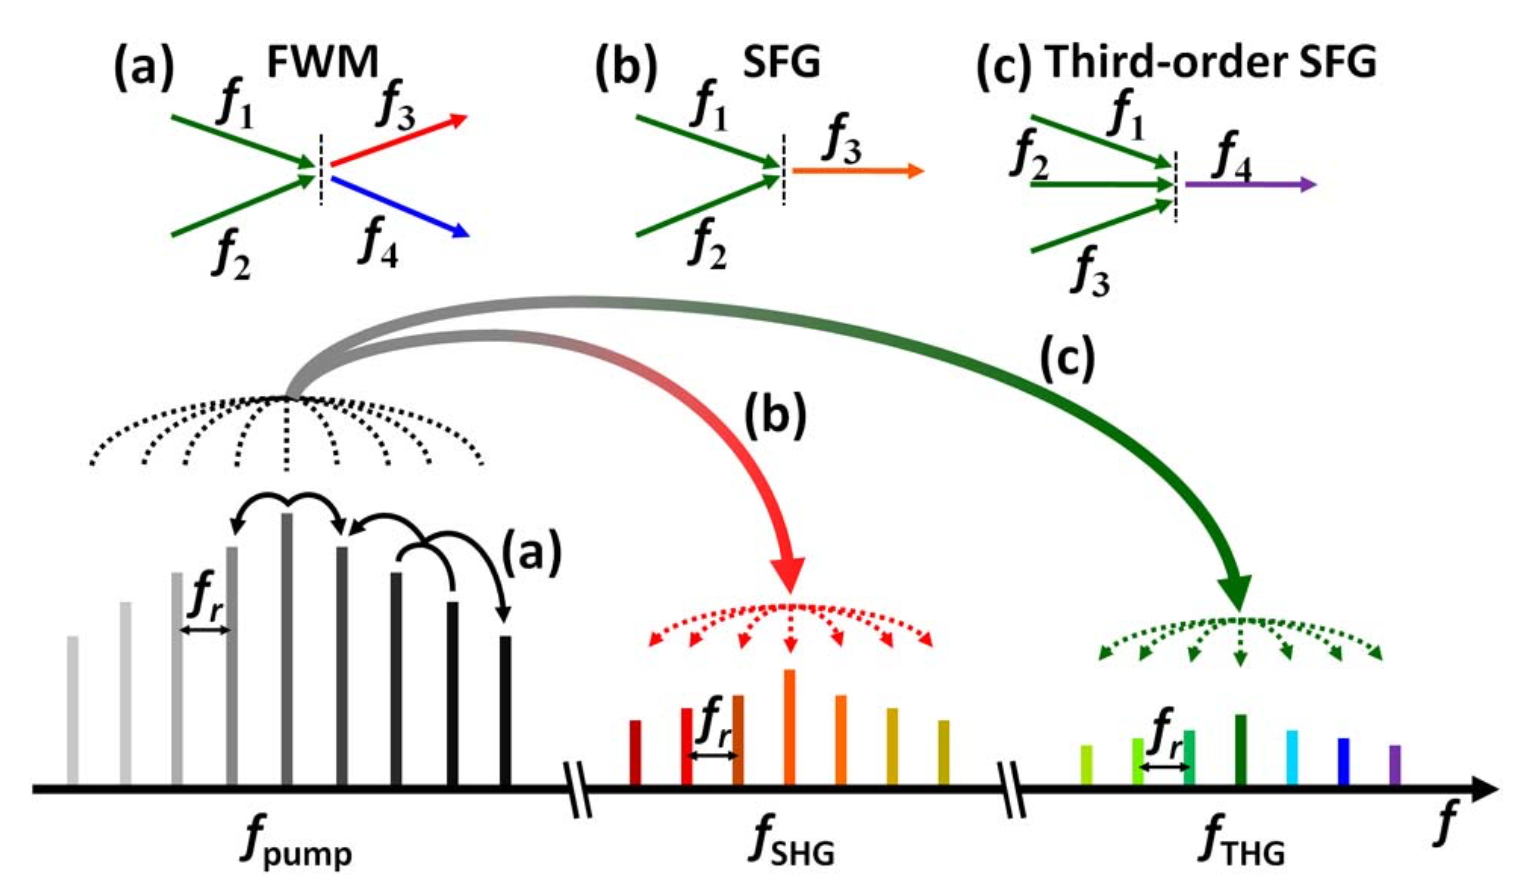
\includegraphics[width=\textwidth]{figures-3/nonlinearity.png}
    \caption[Alumninum nitride frequency conversion diagram]{Diagram of the nonlinear optical processes and frequency conversions that occur within an aluminum nitride waveguide. (a) Side-band generation through cascaded four-wave mixing (FWM) produces a comb centered near the frequency of the pump laser ($f_\mathrm{pump}$). (b) Second-order sum-frequency generation (SFG) produces a comb centered at twice $f_\mathrm{pump}$ (second harmonic generation, SHG). (c) Third-order SFG produces a comb centered at three times $f_\mathrm{pump}$ (third harmonic generation, THG). The repetition rate ($f_r$) within both comb harmonics is the same as in the pump comb. Image reprinted from \cite{jung_green_2014}.}
    \label{fig:nonlinearity}
\end{figure}

Many materials used to develop on-chip waveguides---including silicon [CITATION], silicon nitride [CITATION], aluminum nitride \citep{jung_aluminum_2016}, and lithium niobate [CITATION]---have relatively large $\chi^{(3)}$, meaning that four-wave mixing processes such as third-order sum frequency generation are quite efficient. In addition to straight waveguide applications of third harmonic generation, these materials are also used to produce microresonators (or micro-rings), small rings in which light at only certain discretely-spaced wavelengths resonate. The circumference of the ring dictates the spacing of the resultant frequencies, where from just a single pump laser, numerous comb lines can be produced. When the generation of adjacent comb lines through this process is efficient enough that they begin to cascade, this is known as supercontinuum generation \citep{dudley_supercontinuum_2006}. Supercontinua can produce extremely broadband frequency combs, sometimes even close to octave-spanning, from a single laser source \citep{li_stably_2017, gong_near-octave_2020}.

Alumninum nitride has two strengths compared to these other materials: (1) a strong $\chi^{(2)}$ nonlinearity and (2) a wide band gap \citep{jung_aluminum_2016}. Due to their centrosymmetric structure, silicon and silicon nitride do not display $\chi^{(2)}$ characteristics. Aluminum nitride, on the other hand, can exhibit both three- and four-wave mixing simultaneously. Also, the band gap of aluminum nitride is wider than that of silicon nitride, enabling higher efficiency of blue and ultraviolet light transmission \citep{liu_beyond_2019}. These two properties combined make aluminum nitride an excellent candidate for astro-comb development, which requires continuity and efficiency over the wide bandpass from the ultraviolet through the near-infrared.

The Yale Nanodevices Laboratory has developed a mature nanofabrication process for aluminum nitride that deposits the material with a silicon dioxide cladding onto silicon dioxide or sapphire chips. Using this process, they have fabricated many on-chip aluminum nitride waveguides with varying lengths \citep[300~\si{\micro\meter}--3~\si{\centi\meter};][]{xiong_aluminum_2012}, thicknesses \citep[330--1500~\si{\nano\meter};][]{pernice_second_2012}, and taper geometries \citep{liu_beyond_2019}. These tests demonstrated strong second-order sum frequency generation with differing wavelength-dependent efficiency (phase-matching) depending on the associated geometries. More recently, they have also developed aluminum nitride micro-rings \citep{jung_optical_2013, guo_second-harmonic_2016}, including one that generated a simultaneous green, red, and infrared combs lines that were distinguishable using a $\sim$50,000 resolution spectrograph \citep{jung_green_2014}.

\section{Aluminum Nitride Micro-ring} \label{astro-comb:micro-ring}

The most important aspect of aluminum nitride's potential usability with spectrograph systems such as EXPRES is its ability to convert infrared light efficiently and transparently throughout the entire band-pass of the instrument. As noted in Chapter \ref{intro:wvln_cal}, the Menlo laser frequency comb used with EXPRES has a stated band-pass of 450--750~\si{\nano\meter}, though in practice this has been shown to be closer to 500--720~\si{\nano\meter}. Therefore, demonstration of comb lines that span bluer than 500~\si{\nano\meter} and redder than 720~\si{\nano\meter} would provide evidence for aluminum nitride's ability to simultaneously calibrate the entirety of the EXPRES spectral format.

\begin{figure}
    \centering
    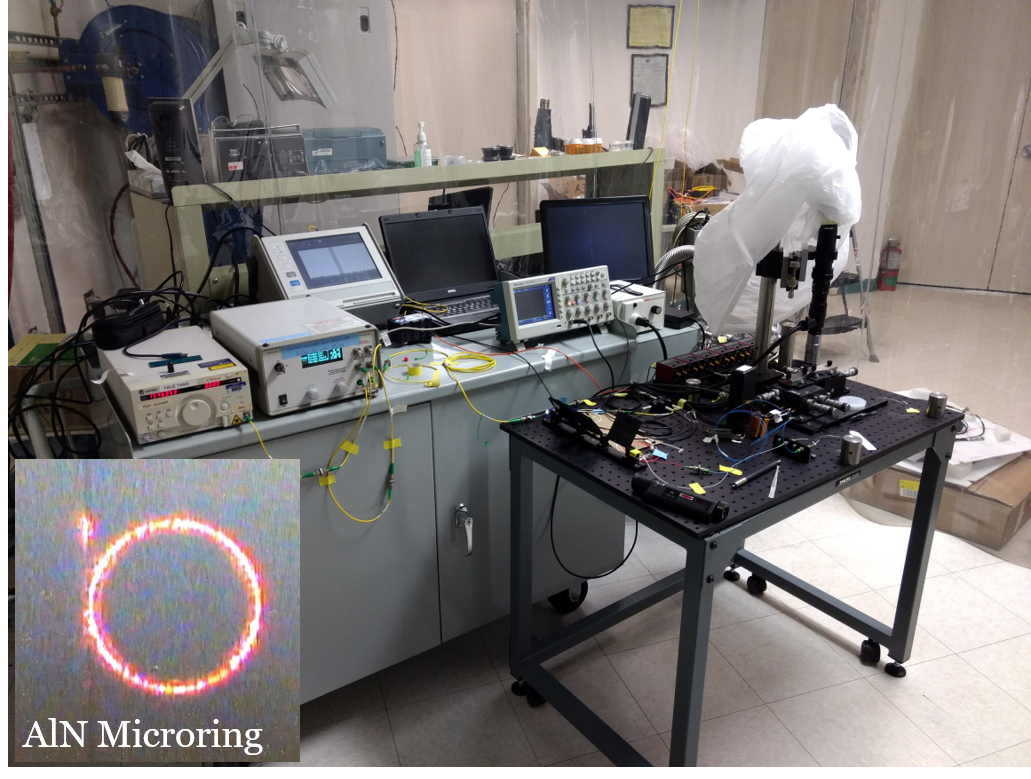
\includegraphics[width=\textwidth]{figures-3/microring-setup.png}
    \caption[Aluminum nitride micro-ring at the Lowell Discovery Telescope]{Image of the aluminum nitride micro-ring setup outside the EXPRES spectrograph room at the Lowell Discovery Telescope. The setup includes a tunable continuous wave near-infrared laser on the very left, immediately next to it is a two stage erbium-doped fiber amplifier, and this is coupled via the components on the optical bench to the aluminum nitride micro-ring. The inset in the bottom left shows a top down view of the micro-ring while it is resonating.}
    \label{fig:microring-setup}
\end{figure}

To do so, we brought an updated version of the aluminum nitride micro-ring introduced in \citet{jung_green_2014} to EXPRES at the Lowell Discovery Telescope during the spectrograph's commissioning in 2018 (Figure \ref{fig:microring-setup}). An amplified tunable continuous-wave near-infrared ($\sim$1550~\si{\nano\meter}) laser is coupled into the device, producing a near-infrared frequency comb that is subsequently doubled ($\sim$780~\si{\nano\meter}) and tripled ($\sim$520~\si{\nano\meter}) throughout the spectral bandwidth of EXPRES. Using a variety of micro-ring geometries---3.4--3.6~\si{\micro\meter} width, 600--800~\si{\nano\meter} gap, 45--60~\si{\micro\meter} radius---we measured the visible frequency comb spectra produced at various resonant pump laser frequencies. In order to highlight certain regions of the spectra without over-saturating other regions on the detector, we used different arrangements of edgepass filters and a wavelength-division multiplexer. Examples of various spectra obtained with EXPRES are shown in Figure \ref{fig:microring-spectra}.

\begin{figure}
    \centering
    \includegraphics[width=\textwidth]{figures-3/microring-spectra.pdf}
    \caption{Spectra of an aluminum nitride micro-ring measured with EXPRES using various configurations of filters and waveguide geometries within three separate wavelength regions of the spectral bandwidth. R, micro-ring radius in \si{\micro\meter}; W, waveguide width in \si{\micro\meter}; G, gap between waveguide and micro-ring in \si{\nano\meter}; $\mathrm{\lambda}$, pump wavelength in \si{\nano\meter}. The blue and orange spectra were taken with a edgepass filter at 650~\si{\nano\meter}. The EXPRES laser frequency comb extends from 5000~\si{\angstrom} to 7200~
    \si{\angstrom}.}
    \label{fig:microring-spectra}
\end{figure}

We found that these configurations of the aluminum nitride waveguide were able to consistently reach from approximately 440~\si{\nano\meter} through the reddest range of EXPRES at 830\si{\nano\meter}. Using the spectral filters, we found relatively high efficiency for both second- and third-harmonic generation of the comb. Unfortunately, this version of the comb does not consistently reach below 440~\si{\nano\meter} except for a few scattered individual lines (see the top plot of Figure \ref{fig:microring-spectra}) likely due to limited broadening of the near-infrared supercontinuum due to the ring. However, the appearance of lines that span redder than 600~\si{\nano\meter} demonstrates aluminum nitride's effectiveness as a frequency doubler and advantage over silicon nitride for astro-comb development.

\section{Electro-optic Modulation Comb} \label{astro-comb:eom}

Rather than rely on a micro-ring to generate a broad enough near-infrared spectrum, we can use near-infrared pulsed laser combs to pump an aluminum nitride straight waveguide, which can be tuned to both broaden and convert the spectrum into the visible regime. \citet{liu_beyond_2019} and \citet{lu_ultraviolet_2020} demonstrated as much with 80~\si{\mega\hertz} femtosecond lasers. However, spectrograph wavelength calibration requires line spacing of more than 10~\si{\giga\hertz}. Therefore, we developed a high-repeition-rate near-infrared electro-optic modulation comb as a pulsed laser source for a straight aluminum nitride waveguide.

\begin{figure}
    \centering
    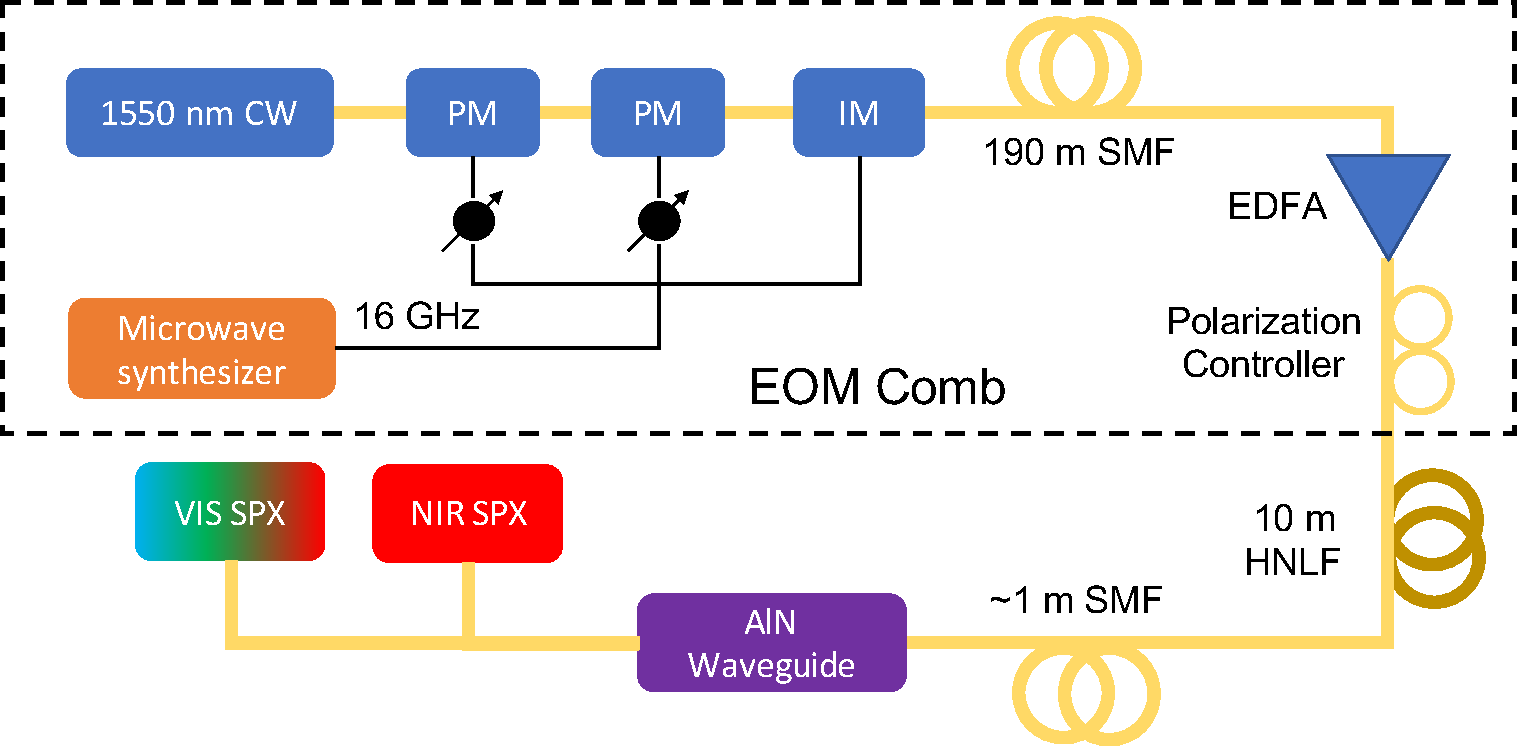
\includegraphics[width=\textwidth]{figures-3/eom-diagram.pdf}
    \caption[Electro-optic modulation comb schematic diagram]{Schematic diagram of the electro-optic modulation comb built for testing with aluminum nitride waveguides. All components within the comb are completely fiber-based, meaning there are no free-space optics until waveguide coupling. EOM, electro-optic modulation; CW, continuous wave laser; PM, polarization modulator; IM, intensity modulator; SMF, single-mode fiber; EDFA, erbium-doped fiber amplifier; HNLD, highly nonlinear fiber; NIR, near-infrared; VIS, visible; SPX, spectrograph.}
    \label{fig:eom-diagram}
\end{figure}

Our electro-optic modulation comb (Figure \ref{fig:eom-diagram}) is designed with a set of off-the-shelf lithium niobate phase (2) and intensity (1) modulators fed by a 1550~\si{\nano\meter} continuous-wave laser. By applying oscillating a voltage across the lithium niobate, we can change the $\chi^{(2)}$ nonlinearity of the material sinusoidally. Depending on the orientation of the lithium niobate crystal structure, either the polarization (which can then be converted to intensity via a polarizer) or phase of propagating light will be modified proportionally to the voltage. The resultant spectrum is a series of side bands surrounding the pump laser frequency separated by the drive frequency of the modulators, which we set to 16~\si{\giga\hertz} using a tunable microwave synthesizer. The relative drive phase of each modulator is matched using independent radio-frequency phase controllers.

The signal coming out of the modulators is chirped, meaning the relative phase of separate frequencies are not aligned, and the intensity of a single pulse is spread out slightly over time. This is corrected by a significant length ($\sim$ 190~\si{\meter}) of single-mode fiber which imparts dispersion compensation opposite that of the chirp. The signal is then amplified using an erbium-doped-fiber amplifier to 3--4~\si{\watt}. In order to broaden the comb before coupling into the waveguide, we send it through 50~\si{\meter} of highly nonlinear silicon fiber. Even though this fiber has nearly zero dispersion, the resultant chirp is again corrected with a short length of single-mode-fiber, minimizing the pulse width at the output of the comb. The optimal length of this final fiber ($\sim$1~\si{\meter}) was determined using a numerical simulation of pulse propagation through the comb. Finally, the optical pulses from this fiber are coupled into an aluminum nitride waveguide using a pair of near-infrared-optimized lenses mounted to a three-axis piezo-controlled alignment stage. Spectra are collected with a combination of near-infrared and visible optical spectrum analyzers.

\begin{figure}
    \centering
    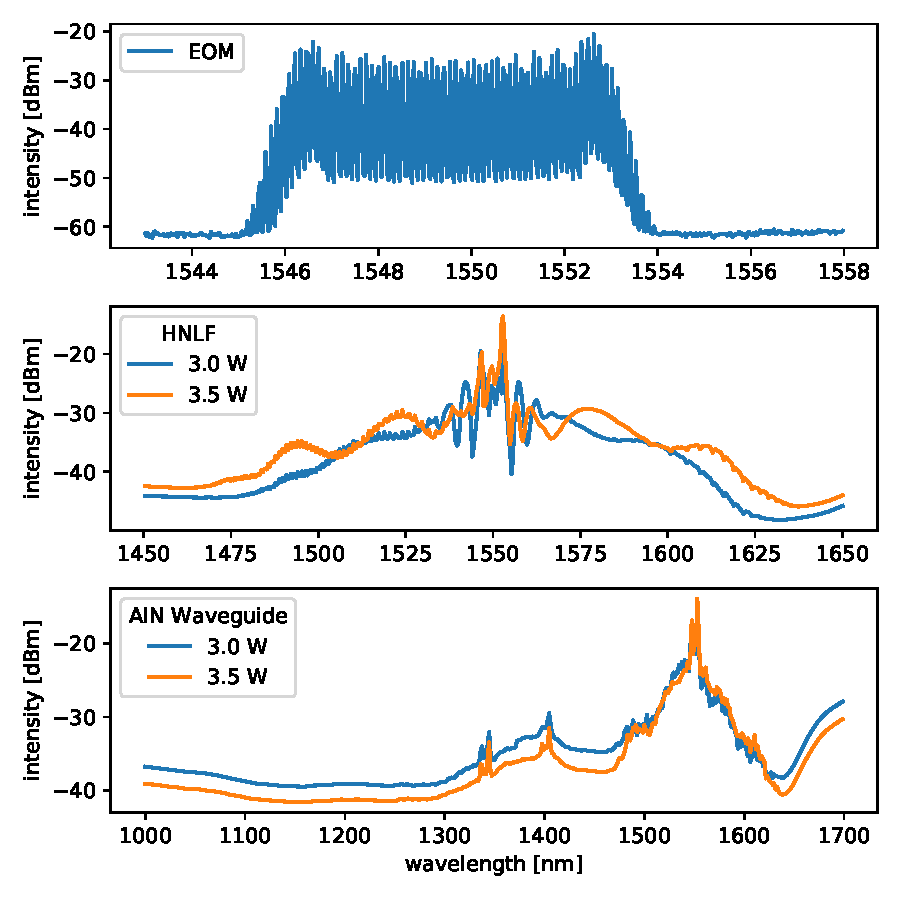
\includegraphics[width=\textwidth]{figures-3/eom-spectra.pdf}
    \caption[Electro-optic modulation comb spectra]{Spectra produce by the electro-optic modulation comb at various points along the optical path. After the electro-optic modulators and single-mode fiber compressor (top), after the highly nonlinear fiber (middle), and after the aluminum nitride waveguide (bottom). Two different amplification power levels are shown for the middle and bottom plots.}
    \label{fig:eom-spectra}
\end{figure}

Output spectra at various stages along the electro-optic modulation comb are shown in Figure \ref{fig:eom-spectra}. Immediately after the electro-optic modulators, the comb bandwidth is approximately 6~\si{\nano\meter}. This is extended to about 100~\si{\nano\meter}, from 1500~\si{\nano\meter} to 1600~\si{\nano\meter}, after amplification and then broadening from the highly nonlinear fiber. The spectrum is not broadened much further by the aluminum nitride waveguide, with some sum-frequency generation occurring around 1400~\si{\nano\meter} and 1340~\si{\nano\meter}. Although not shown here, the 100~\si{\nano\meter} comb around the pump frequency was efficiently converted to a 50~\si{\nano\meter} comb around 780~\si{\nano\meter} and a 33~\si{\nano\meter} comb around 520~\si{\nano\meter}.

\begin{figure}
    \centering
    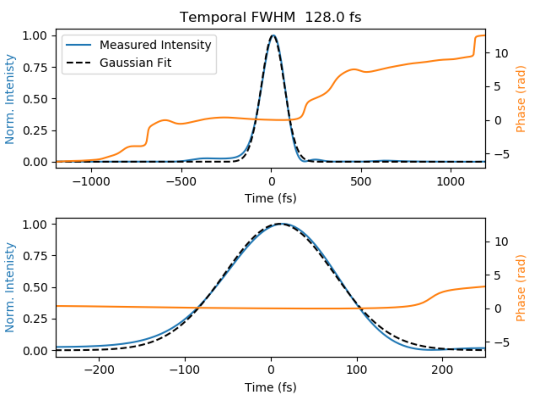
\includegraphics[width=\textwidth]{figures-3/eom-pulse.pdf}
    \caption[Electro-optic modulation comb pulse width]{Pulse width of the electro-optic modulation comb at the point of coupling with the aluminum nitride waveguide. The bottom plot is the same data zoomed in. Gaussian fitting of the line reveals a full-width-half-maximum of about 128~\si{\femto\second}.}
    \label{fig:eom-pulse}
\end{figure}

Measuring the pulse width of the light coupled into the waveguide (Figure \ref{fig:eom-pulse}, we find that it is longer than 120~\si{\femto\second}. Similar electro-optic modulation combs combined with silicon nitride waveguides were able to achieve sub-100~\si{\femto\second} pulses \citep{carlson_ultrafast_2017, obrzud_visible_2019}, meaning our system is likely not tuned enough for maximal pulse compression. We even tested our system on a silicon nitride waveguide similar to the one used by \citet{carlson_ultrafast_2017}, but were not able to achieve an octave-spanning comb. By decreasing the width of the pulse, we could increase the peak power of the signal entering the aluminum nitride waveguide, thereby better exciting its nonlinearity and more likely producing a broader supercontinuum in the near-infrared.

\section{Summary and Discussion}

In summary, we were able to demonstrate the efficacy of aluminum nitride as a candidate for application to radial-velocity spectroscopy wavelength calibration. The aluminum nitride micro-ring tested on EXPRES yielded lines over almost all of the instrument's spectral bandwidth from 440~\si{\nano\meter} to above 820~\si{\nano\meter}, while even occasionally producing lines in the near-ultraviolet. An electro-optic modulation comb, designed to couple into a straight aluminum nitride waveguide, was able to produce a fairly broadband (VALUES) near-infrared frequency comb that could be doubled and tripled to cover the visible regime with significantly less complexity than mode-locked laser frequency comb systems. Unfortunately, broadening of this comb did not reach near-octave bandwidth, likely due to insufficient pulse compression before coupling into the waveguide, meaning a completely viable visible astro-comb design was not achieved.

Although this work was not yet able to generate a extremely broadband visible frequency comb, promising results have been coming from a team at the University of Geneva \citep{obrzud_visible_2019}. Using a completely fiber-based electro-optic system almost identical to the one presented here \citep{obrzud_microphotonic_2019}, they demonstrated complete wavelength coverage from 400--600~\si{\nano\meter} through a silicon nitride waveguide, further demonstrating the material's utility for triple sum-frequency generation. The only other difference between our designs is that they use a chirped fiber Bragg grating over our long single-mode fiber. However, even when we replaced the long single-mode fiber with a dispersion-controller, we were still not able to achieve enough spectral broadening. It therefore appears that the relative lengths of our highly nonlinear fiber and dispersion compensating fibers need to be better tuned to minimize the pulse width before coupling into the waveguide. I would recommend using a longer highly nonlinear fiber to increase this first stage of broadening and then re-optimizing the length of the final single-mode fiber compressor to match the new dispersion profile.

Considering silicon nitride does not have strong second harmonic generation, however, there still remains a space for aluminum nitride within visible radial-velocity spectroscopy. If we could properly tune the electro-optic setup described here, in principle, the combined comb would produce the same 400--600~\si{\nano\meter} blue-green comb as well as a simultaneous 600-900~\si{\nano\meter} red comb. The blue comb may also extend a bit further into the ultraviolet due to the larger band gap. A frequency comb produced by such a device would easily cover the entirety of the EXPRES spectral bandwidth. Unfortunately, due to circumstances created by the pandemic, further astro-comb tuning was not possible within the time-frame of the writing of this thesis.

One possible avenue for future exploration with this technology would be to combine a $\sim$16~\si{\giga\hertz} micro-ring (either aluminum nitride or lithium niobate) with the electro-optic modulation comb. Naturally, this will add more complexity into the system, since the the continuous-wave laser and microwave synthesizer frequency would need to be tuned to match resonance with the micro-ring. However, this may enable greater efficiency in the spectral broadening of the near-infrared comb before converting to visible wavelengths. By continuing research along this track, we may someday soon be able to design an astro-comb completely contained on a single chip-based aluminum nitride waveguide.

Special thanks to Alex Bruch for his significant guidance in learning the ins and outs of nonlinear optics, for contributing his simulation code to this chapter, for joining me in collecting micro-comb data with EXPRES, and for helping me to develop the electro-optic modulation comb. I would also like to thank Zheng Gong for his help in testing the electro-optic modulation comb. I would finally like to thank Scott Diddams and Stephanie Leifer for their guidance through the electro-optic modulation prototyping process.